\newpage
\section{Theoretical Analysis}
\label{sec:analysis}

\subsection{Exercise 1}
\label{Analysis Exercise 1}

%---------------Theoretical Analysis Exercise 1--------------------------------------------------------%
\begin{figure}[!ht] \centering
\caption{Representation of mesh currents in the circuit.}
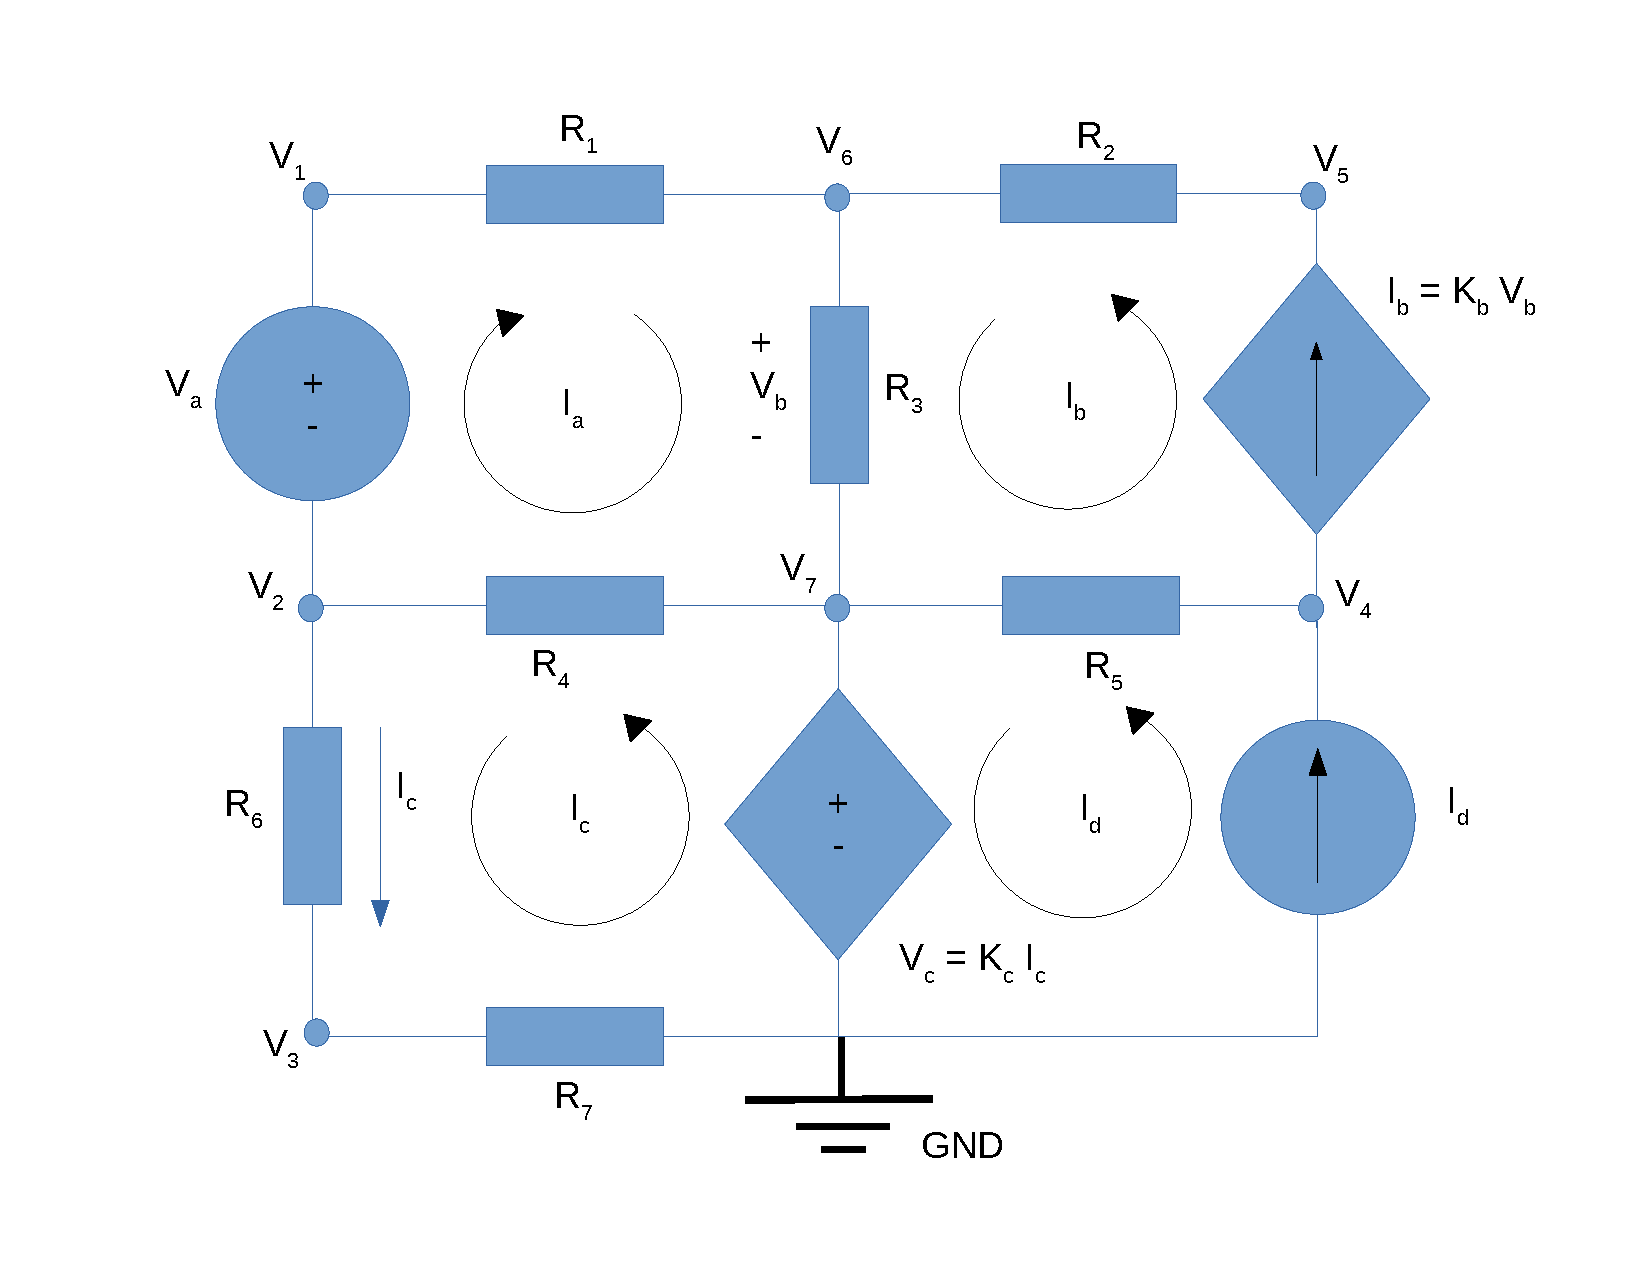
\includegraphics[width=0.8\linewidth]{circuit_mesh.pdf}
\label{fig:meshcurrents}
\end{figure}

%---------------Theoretical Analysis Exercise 1--------------------------------------------------------%
 
The first thing which must be noticed is that there is an independent voltage source ($V_s$) and a linear current controlled voltage source ($V_d$) in this circuit. Knowing that a nodal analysis can't include the analysis of nodes that are connected to voltage sources, it becomes clear that is useless to analyze nodes 1 and 4 (connected to $V_s$) and also nodes 5 and 8 (connected to $V_d$) using this method.

From figure~\ref{fig:??}, we can easily conclude that there are 11 unknown variables: $V_b$, $I_b$, $V_d$, $I_d$, $V_1$, $V_2$, $V_3$, $V_5$, $V_6$, $V_7$ and $V_8$. In this exercise, $V_s$ is constant and the capacitor is assumed to be also constant and fully charged, meaning that the current $I_c$ is 0 (open circuit behavior).

For the node analysis, it is necessary to consider 7 linearly independent equations to reach all the values corresponding to the voltages in each node and consequently solve the circuit. As referred above, it is possible to use the nodal method to analyze nodes 2, 3, 6 and 7.

We begin by establishing the following equations, being that equations ~\ref{eq:given11} and ~\ref{eq:given12} were given by the professor. Equation ~\ref{eq:vb1} was obtained by relating the voltage difference between nodes 2 and 5 to the voltage $V_b$. Finally, by using Ohm's Law for resistor $R_6$ and remembering that $V_4$ is null, we get the last equation (\ref{eq:id1}) for $I_d$.

\begin{equation}
  I_{b} = K_{b}V_{b} ,
  \label{eq:given11}
\end{equation}

\begin{equation}
  V_{d} = K_{d}I_{d} ,
  \label{eq:given12}
\end{equation}

\begin{equation}
  V_{b} = V_{2} - V_{5} ,
  \label{eq:vb1}
\end{equation}

\begin{equation}
  I_{d} = -V_{7}G_{6} ,
  \label{eq:id1}
\end{equation}

The equation written below (\ref{eq:node11}) is a direct consequence of our choice of connecting node 4 to the ground (GND), because this choice makes evident that the value of $V_4$ is 0 and then:
\begin{equation}
  V_{1} - V_{s} = 0,
  \label{eq:node11}
\end{equation}

%he equation below (\ref{eq:node3a}) was figured out by using Kirchoff's Current Law for node 2 and Ohm's Law for the resistors $R_6$ and $R_7$. To correctly use the Ohm's Law for the resistor $R_7$, it is important to remember that the value we assigned to $V_4$ is 0. USAR QUANDO V4

By analysing node 2 using Kirchoff's Current Law and Ohm's Law for the resistors $R_1$, $R_2$ and $R_3$, we get the following equation:

\begin{equation}
  (V_{3} - V_{1})G_{1} + (V_{2} - V_{3})G_{2} + (V_{2} - V_{5})G_{3}= 0,
  \label{eq:node12}
\end{equation}

The following equation (\ref{eq:node13}), in which was also used Kirchoff's Current Law and Ohm's Law for resistor $R_2$, refers to node 3. Here we consider the given equation ~\ref{eq:given11} and the equation ~\ref{eq:vb1} to substitute the current $I_b$.

\begin{equation}
  (V_{3} - V_{2})G_{2} - (V_{2} - V_{5})K_{b} = 0,
  \label{eq:node13}
\end{equation}

For node 6, the ensuing equation (\ref{eq:node16}) was figured out by resorting to Ohm's Law for the resistor $R_5$ and Kirchoff's Current Law. Equations ~\ref{eq:given11} and~\ref{eq:vb1} were once again used to avoid using $I_b$. Remember that, for this exercise, $I_c$ is null.

\begin{equation}
  (V_{6} - V_{5})G_{5} + (V_{2} - V_{5})K_{b} = 0,
  \label{eq:node16}
\end{equation}

Finally, for node 7, Kirchoff's Circuit Law and Ohm's Law (for resistors $R_6$ and $R_7$) were used to establish the following mathematical relation:

\begin{equation}
  V_{7}G_{6} + (V_{7} - V_{8})G_{7} = 0,
  \label{eq:node17}
\end{equation}

Since there are 7 unkown varibles, we need two more equations. The first one (\ref{eq:vd1}) is obtained by relating $V_d$ to the voltage difference in nodes 5 and 8 and replacing $V_d$ for the equations~\ref{eq:given12} and~\ref{eq:id1}.

\begin{equation}
  -V_{7}G_{6}K_{d} - (V_{5} - V_{8}) = 0,
  \label{eq:vd1}
\end{equation}

Ultimately, to discover the last equation, there are some theoretical concepts that must be considered. Kirchoff's Current Law implies that there is no current stuck at any node. It is also known that neither voltage sources nor resistors retain current. Then, any branch that only contains one of the said elements does not retain current as well. Merging the two branches placed on the left side of circuit (branch containing $V_s$ with branch containing $R_6$) and calling Supernode to the result of this merger, it is still true that no current is retained in the Supernode. Then, considering that all unkown currents are diverging from the nodes, the resultant equation (\ref{eq:supernode1}) is the one written right below.

\begin{equation}
  (V_{1} - V_{2})G_{1} - V_{5}G_{7} - V_{7}G_{6} = 0,
  \label{eq:supernode1}
\end{equation}

A system with the 7 linearly independent equations and 7 variables (regarding the voltage in each node) is, of course, possible to solve but not easy (and certainly not pratical) to deal with. The following matrix equation (\ref{eq:nodalmatrix1}) summarizes the 7 referred equations so it is easier to read and to instantaneously solve (by using Octave).
\begin{equation}
\left[ \begin{array}{ccccccc} 
		1 & 0 & 0 & 0 & 0 & 0 & 0 \\ 
		-G_1 & G_1+G_2+G_3 & -G_2 & -G_3 & 0 & 0 & 0 \\
		0 & -G_2-K_b & G_2 & K_b & 0 & 0 & 0 \\ 
		0 & K_b & 0 & -K_b-G_5 & G_5 & 0 & 0  \\ 
		0 & 0 & 0 & 0 & 0 & G_6+G_7 & -G_7  \\ 
		G_1 & -G_1 & 0 & -G_4 & 0 & -G_6 & 0  \\ 
		0 & 0 & 0 & -1 & 0 & -K_dG_6 & 1 \\ 

\end{array} \right]
\times \left[ \begin{array}{c} V_1 \\ V_2 \\ V_3 \\  V_5 \\ V_6 \\ V_7 \\ V_8 \end{array} \right] =
\left[ \begin{array}{c} V_s \\ 0 \\ 0 \\ 0 \\ 0 \\ 0 \\ 0  \end{array} \right]
\label{eq:nodalmatrix1}
\end{equation}

To find all the required branches' currents we can use Ohm's Law for each resistor, which can be seen in equations~\ref{eq:ohm11} to~\ref{eq:ohm17}: Now we no longer consider the currents to be diverging from the nodes, but assume the directions shown in figure~\ref{fig:??}.

\begin{equation}
  R_1[i] = \frac{V_1 - V_2}{R_1},
  \label{eq:ohm11}
\end{equation}

\begin{equation}
  R_2[i] = \frac{V_2 - V_3}{R_2},
  \label{eq:ohm12}
\end{equation}

\begin{equation}
  R_3[i] = \frac{V_5 - V_2}{R_3},
  \label{eq:ohm13}
\end{equation}

\begin{equation}
  R_4[i] = \frac{V_5}{R_4},
  \label{eq:ohm14}
\end{equation}

\begin{equation}
  R_5[i] = \frac{V_6 - V_5}{R_5},
  \label{eq:ohm15}
\end{equation}

\begin{equation}
  R_6[i] = -\frac{V_7}{R_6},
  \label{eq:ohm16}
\end{equation}

\begin{equation}
  R_7[i] = \frac{V_7 - V_8}{R_7},
  \label{eq:ohm17}
\end{equation}

\begin{table}[!ht]
\centering
\begin{tabular}{ |c|c|} 
 \hline
 {\bf Node} & {\bf Voltage[V]} \\ 
 \hline\hline
  $V_b$ & \partialinput{1}{1}{theoretical_1.tex}\\ 
 \hline
  $V_d$ & \partialinput{2}{2}{theoretical_1.tex} \\ 
 \hline
 $V_1$ & \partialinput{3}{3}{theoretical_1.tex} \\ 
 \hline
 $V_2$ & \partialinput{4}{4}{theoretical_1.tex} \\ 
 \hline
 $V_3$ & \partialinput{5}{5}{theoretical_1.tex} \\ 
 \hline
 $V_5$ & \partialinput{6}{6}{theoretical_1.tex} \\ 
 \hline
 $V_6$ & \partialinput{7}{7}{theoretical_1.tex} \\ 
\hline
 $V_6$ & \partialinput{8}{8}{theoretical_1.tex} \\ 
 \hline
 $V_8$ & \partialinput{9}{9}{theoretical_1.tex} \\
 \hline
\end{tabular}
\caption{Voltage and Current values(Exercise 1)}
\begin{tabular}{ |c|c|} 
 \hline
 {\bf Branch} & {\bf Current[A]}\\ 
 \hline\hline
 $I_b$ & \partialinput{10}{10}{theoretical_1.tex} \\ 
 \hline
 $I_c$ & \partialinput{11}{11}{theoretical_1.tex} \\
 \hline
 $R_6 = I_d$ & \partialinput{12}{12}{theoretical_1.tex} \\
 \hline
 $R_1$ & \partialinput{13}{13}{theoretical_1.tex} \\ 
 \hline
  $R_2$ & \partialinput{14}{14}{theoretical_1.tex} \\ 
 \hline
  $R_3$ & \partialinput{15}{15}{theoretical_1.tex} \\  
 \hline
 $R_4$ & \partialinput{16}{16}{theoretical_1.tex} \\ 
 \hline
 $R_5$ & \partialinput{17}{17}{theoretical_1.tex} \\  
 \hline
  $R_7$ & \partialinput{19}{19}{theoretical_1.tex} \\  
 \hline
\end{tabular}
\label{table:theoretical_1}
\end{table}

%\begin{figure}[!ht] \centering
%\caption{Final solution of $v_6(t)$ and $v_s(t)$ in the interval $[-5,20]ms$}
%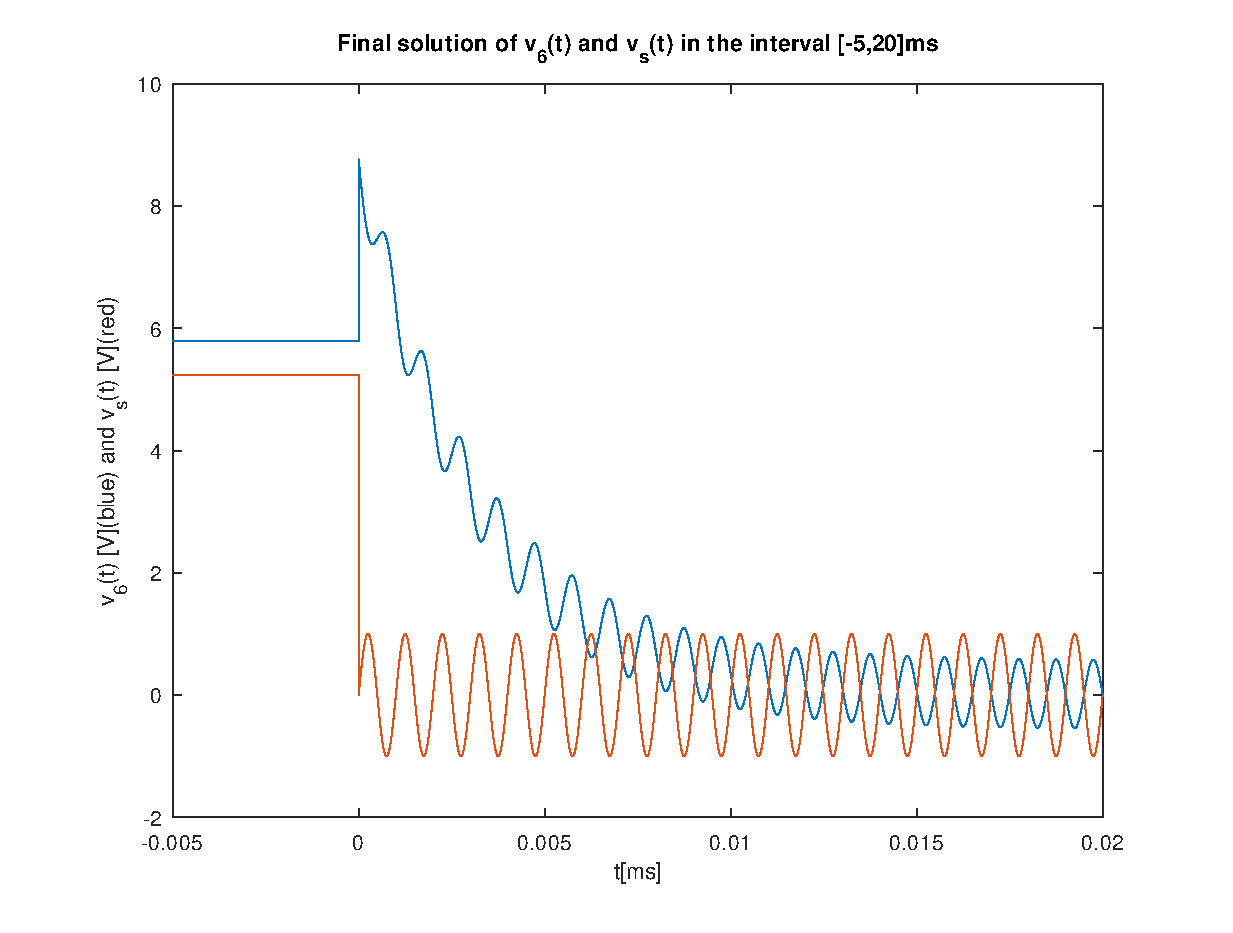
\includegraphics[width=0.8\linewidth]{theoretical_5.eps}
%\label{fig:circuit}
%\end{figure}






